\chapter{Architecture}
\section{Fix Step}
By default, the CORDIC algorithm converges only for input angles within the range \( (-99.7^\circ, 99.7^\circ) \).
To address this limitation and enable the algorithm to handle arbitrary input angles, we introduced an \textbf{initial correction step}. This step adjusts the input angle to bring it into the principal range of the algorithm. The adjustment ensures that the CORDIC algorithm works seamlessly for all input angles, not just those within the default convergence range.
\[
    x_0 = -y_{\text{input}} \cdot d_{\text{input}}
\]
\[
    y_0 =  x_{\text{input}} \cdot d_{\text{input}}
\]
\[
    z_0 = -\frac{\pi}{2} \cdot d_{\text{input}}
\]

Additionally, since the iterative process of the CORDIC algorithm introduces a scaling factor \( A_n \), we normalize the final result by dividing \( \rho \) (the magnitude) by \( A_n \).

\section{Algorithm implementation}
\label{sec:algorithm_implementation}

With reference to the Equations \ref{eq:CORDIC}, the combinatorics of a single step is given by the following block diagram:

\begin{figure}[H]
    \centering
    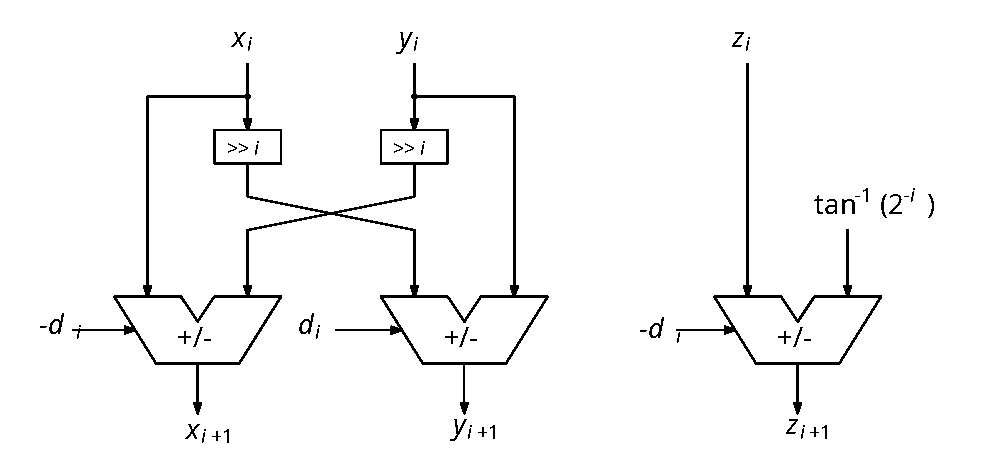
\includegraphics[width=0.7\textwidth]{images/Architecture/basic_CORDIC.pdf}
    \caption{Block diagram of a single step of CORDIC}
    \label{fig:basic_CORDIC}
\end{figure}

Since the CORDIC algorithm typically converges at a rate of one bit per iteration, the number of steps is predetermined at design time based on data representation. For this reason, a possible implementation of CORDIC involves a series of \( n \) combinatorics as shown in Figure \ref{fig:basic_CORDIC}. The resulting combinatorics between input and output registers will assume the following form:

\begin{figure}[H]
    \centering
    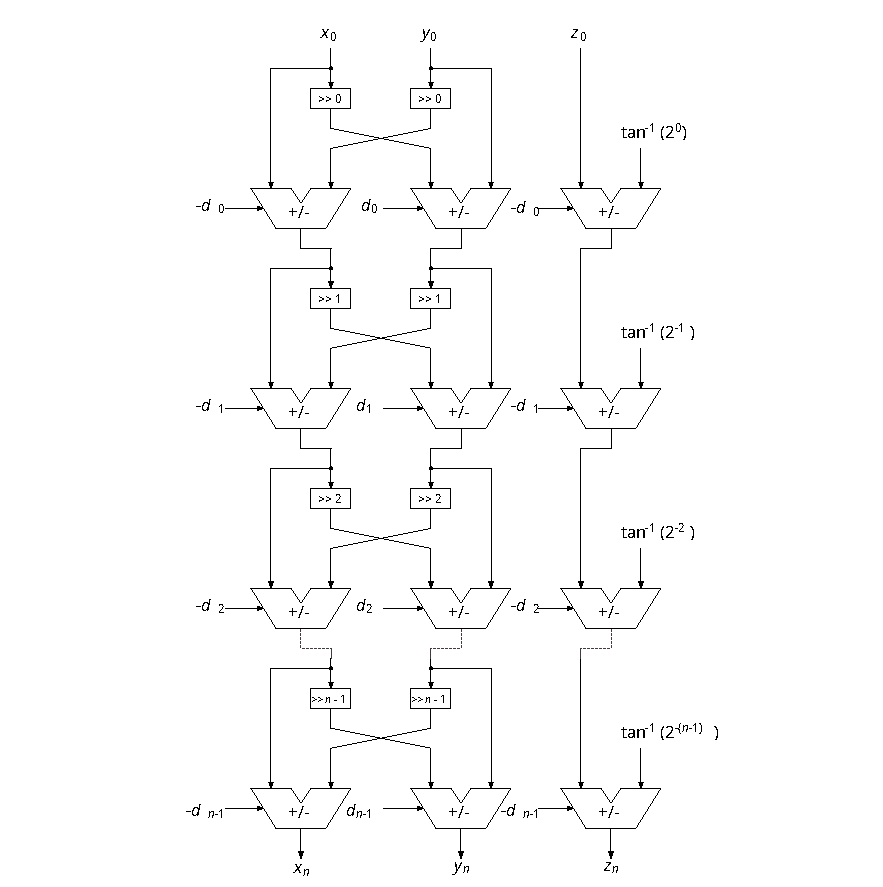
\includegraphics[width=0.9\textwidth]{images/Architecture/pipelined_CORDIC.pdf}
    \caption{Block diagram of the full combinatorics of CORDIC algorithm}
    \label{fig:pipeline_CORDIC}
\end{figure}

Assuming the shift operation has no cost, the logic required will be composed by \(3 \cdot N\) adders, where \(N\) represents the number of iterations needed for convergence. Additionally, the function will go through \(N\) levels of logic. Solutions designed in this way tend to have a long critical path, resulting in a low clock frequency for the network.

To address this limitation, pipelined solutions are generally preferred. By introducing three registers between each step of the process, the throughput of the design remains unchanged. However, the critical path reduces to:

\[
T_{\text{critical}} = T_{c \to q} + T_{\text{prop}} + T_{\text{setup}},
\]

where \(T_{c \to q}\) is the clock-to-Q delay of the flip-flop, \(T_{\text{prop}}\) is the propagation delay of the combinatorial logic which, this time, is just a single level of adder, and \(T_{\text{setup}}\) is the setup time of the next flip-flop.

Although this modification improves the clock speed, it introduces new trade-offs: The delay for processing a single input becomes \(N \cdot T_{\text{clk}}\). More critically, the cost in terms of area occupation and number of components increases significantly, as \(3 \cdot N\) additional registers are inserted into the design. This also negatively impacts power consumption. Hybrid solutions, where registers are placed every 2 or 3 levels of logic, are also commonly adopted nowadays to balance clock speed, area efficiency, and power consumption.

The solution we adopted takes advantage of the recursive nature of the CORDIC equations by slightly modifying the single step and incorporating a feedback loop. This design choice ensures a small critical path, allowing for a high clock frequency while minimizing area occupation, cost, and power consumption:

\begin{figure}[H]
    \centering
    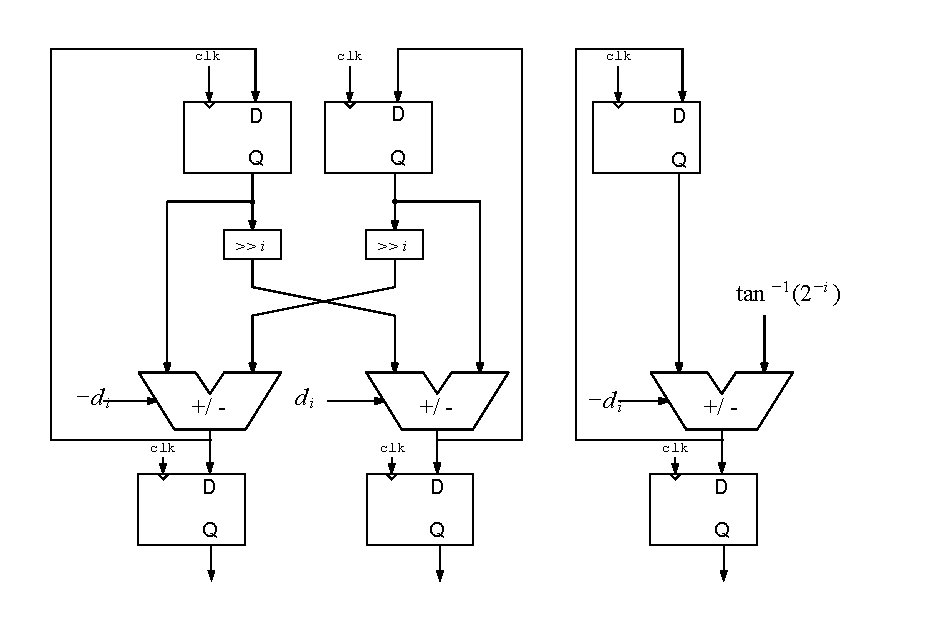
\includegraphics[width=0.7\textwidth]{images/Architecture/actual_CORDIC.pdf}
    \caption{Block diagram of a single step CORDIC with feedback loop}
    \label{fig:actual_CORDIC}
\end{figure}


This approach was chosen with a specific scenario in mind: the CORDIC algorithm acting as an on-board accelerator. In such a scenario, a smaller design with lower power consumption is highly desirable, as it facilitates integration without significantly affecting the board's utilization, heat dissipation, or energy requirements.

In order to achieve this, we will adopt a Finite State Machine (FSM) with a control part, which includes a status register, and an operational part dedicated to performing the necessary calculations.
\vspace{10pt}
\begin{center}
    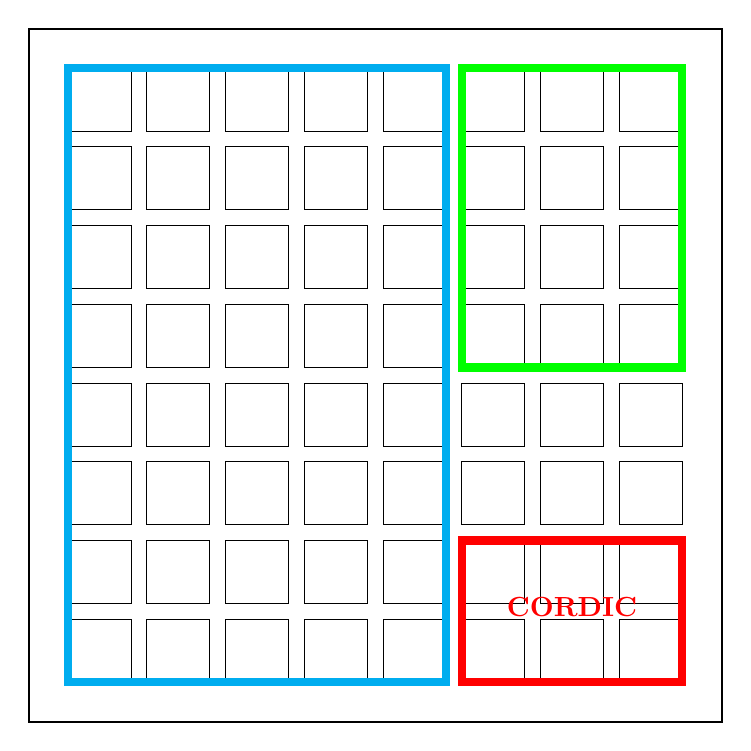
\begin{tikzpicture}
    
        % Draw the FPGA square
        \draw[thick] (-0.5,-0.5) rectangle (8.3,8.3);
        
        % Define the grid size and spacing
        \def\squaresize{0.8} % Size of each square
        \def\margin{0.2}     % Margin between squares
        
        % Draw the grid inside the FPGA
        \foreach \x in {0, 1, ..., 7} {
            \foreach \y in {0, 1, ..., 7} {
                \draw (\x * \squaresize + \x * \margin, \y * \squaresize + \y * \margin)
                    rectangle ++(\squaresize, \squaresize);
            }
        }
        
        % Outline colored blocks to represent usage
        \draw[cyan, thick, line width=3pt] (0 * \squaresize + 0 * \margin, 0 * \squaresize + 0 * \margin)
            rectangle ++(5 * \squaresize + 4 * \margin, 8 * \squaresize + 7 * \margin);
        \draw[green, thick, line width=3pt] (5 * \squaresize + 5 * \margin, 4 * \squaresize + 4 * \margin)
            rectangle ++(3 * \squaresize + 2 * \margin, 4 * \squaresize + 3 * \margin);
        
        % Highlight the small CORDIC square
        \draw[red, thick, line width=3pt] (5 * \squaresize + 5 * \margin, 0 * \squaresize + 0 * \margin)
        rectangle ++(3 * \squaresize + 2 * \margin, 2 * \squaresize + 1 * \margin);
        \node[red] at (6.5 * \squaresize + 6 * \margin, 1.2 * \squaresize) {\textbf{CORDIC}};
        
    \end{tikzpicture}
    \vspace{10pt}
    \captionof{figure}{Schematic representation of an FPGA. The grid represents the available logic blocks, with coloured outlines indicating resource usage. The CORDIC block, highlighted in red, is a small portion of the total FPGA area.}
\end{center}
\vspace{10pt}

It is true that this design results in a delay of \(N \cdot T_{\text{clk}}\) for each operation and reduces throughput to \(1/N\) (processing one input every \(N\) clock cycles). However, these trade-offs are justified by the need to prioritize compactness and efficiency over throughput, aligning with the intended use case of the CORDIC as an auxiliary accelerator.

\section{Data Representation}

To implement the CORDIC algorithm, we used fixed-point arithmetic for the input and intermediate values. Specifically:

\begin{itemize}
    \item \( x \), \( y \) : signed 16-bit fixed-point representation with 8 bits allocated for the fractional part.
    \item \( \rho \) : unsigned 16-bit fixed-point representation with 8 bits allocated for the fractional part.
    \item \( z \), \( \theta \) : signed 16-bit fixed-point representation with 13 bits allocated for the fractional part. This decision was made because they always lie within the range \( [-\pi, \pi] \), and the additional fractional bits ensure high angular precision.
    \item For the intermediate calculations a 24-bit representation was used to minimize truncation errors during the iterative process.
    \item All the inputs and the outputs are limited to 16 bits due to the I/O pin constraints of the Zybo board.
\end{itemize}

The number of iterations for the CORDIC algorithm was set to 16, as this provides a high level of precision while balancing computational efficiency. Beyond 16 iterations, the precision gained decreases significantly.

\section{Module Precision}
The parameter \( \rho \) is represented as unsigned with a UQ8.8 fixed-point format. During intermediate calculations, it uses a UQ10.14 format instead of UQ8.16 in order to prevent overflow. Specifically, the two additional integer bits account for cases like \( x = 127 \) and \( y = 127 \), where the output, before normalization, is

\[
\text{Output} = A_n \cdot \sqrt{2} \cdot 127,
\]

with \( A_n \approx 1.6467605 \). Substituting, the value is approximately 

\[
\text{Output} \approx 1.6467605 \cdot 1.4142135 \cdot 127 \approx 295.342.
\]

This value exceeds the UQ8.16 range but fits within UQ10.14. After normalization, the output is scaled by \( \frac{1}{A_n} \approx 0.607252 \) and then converted to the Q8.8 format by truncation of the least significant bits (LSBs).

\section{Phase Precision and Error Analysis}
Focusing on the phase, \( \theta \) us represented as signed with Q3.13 fixed-point format. During intermediate calculations it uses a Q3.21 fixed-point format. Assuming no error on the input, the values of \( \text{atan}(2^{-1}) \) in Q3.21 format have an absolute error \( \epsilon_a \) of \(2^{-21}\). Over the course of 16 iterations, the accumulated error \( \epsilon_M \) becomes:

\[
    \epsilon_M = \epsilon_a * 16 = 2^{-21} * 2^{4} = 2^{-17}
\]

Since the final result is truncated to Q3.13, which involves discarding the LSBs, the accumulated error from the iterative sums becomes negligible. This ensures that the phase computation maintains high precision.